\documentclass[border=12pt]{standalone}
\usepackage{amssymb}
\usepackage{amsmath}
\usepackage{tikz}
\usetikzlibrary{arrows.meta, decorations.pathreplacing, calc, positioning}

% Project palette (matches covering_diagram.tex)
\definecolor{cnavy}{HTML}{0E2747}
\definecolor{corange}{HTML}{E8573F}
\definecolor{cgreen}{HTML}{3B9B6D}
\definecolor{cslate}{HTML}{5B6680}
\definecolor{cmuted}{HTML}{9B9484}
\definecolor{ccream}{HTML}{FAFAF6}

\begin{document}
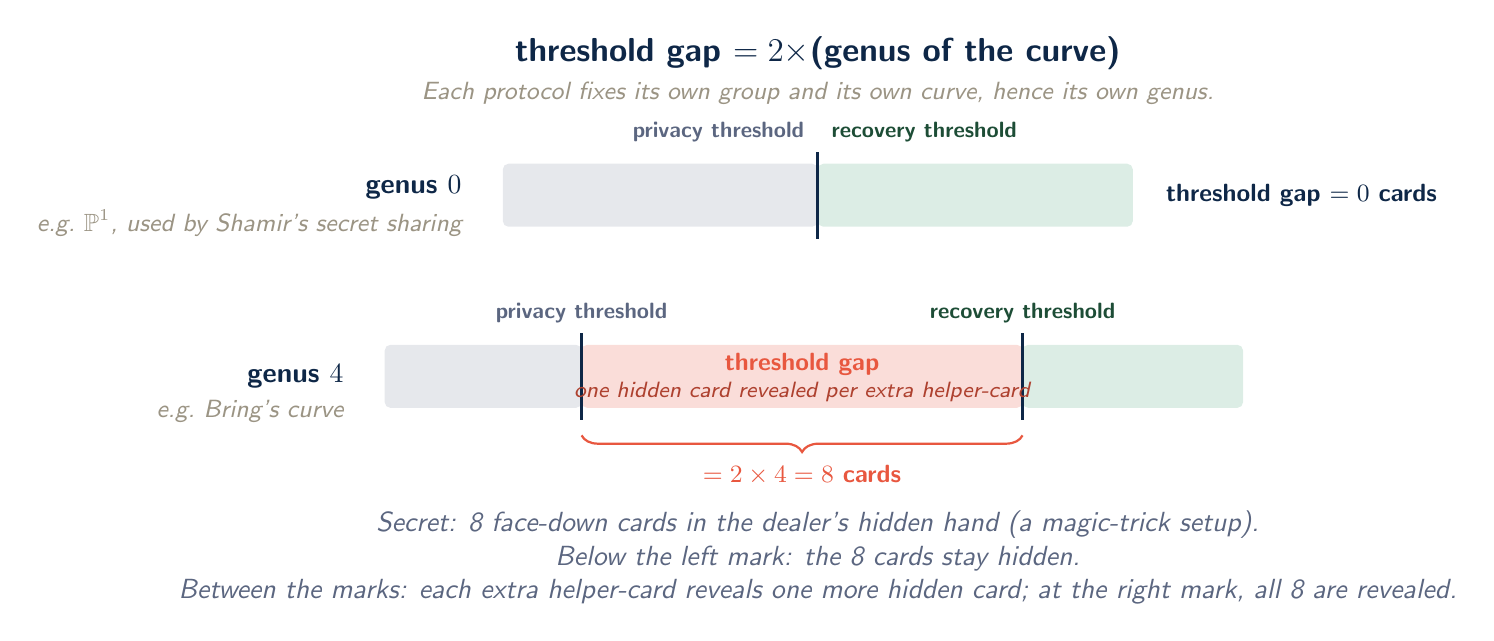
\begin{tikzpicture}[font=\sffamily]

% Headline: the formula being illustrated
\node[cnavy, font=\sffamily\bfseries\large] at (6.0, 5.8)
  {threshold gap $= 2 \times $(genus of the curve)};
\node[cmuted, font=\sffamily\itshape\small] at (6.0, 5.3)
  {Each protocol fixes its own group and its own curve, hence its own genus.};

% ============================================================
% Row 1: genus 0 (collapsed threshold).
% Single mark at x = 6.0. Privacy and recovery coincide.

% Privacy zone (slate-blue), to the left of mark
\fill[cslate!15, rounded corners=2pt] (2.0, 3.6) rectangle (6.0, 4.4);
% Recovery zone (green), to the right
\fill[cgreen!18, rounded corners=2pt] (6.0, 3.6) rectangle (10.0, 4.4);
% Mark
\draw[cnavy, line width=1.2pt] (6.0, 3.45) -- (6.0, 4.55);

% Threshold labels above the mark
\node[cslate, font=\sffamily\bfseries\footnotesize, anchor=south east] at (5.95, 4.55)
  {privacy threshold};
\node[cgreen!50!black, font=\sffamily\bfseries\footnotesize, anchor=south west] at (6.05, 4.55)
  {recovery threshold};

% Row label
\node[cnavy, font=\sffamily\bfseries, anchor=east] at (1.6, 4.1) {genus $0$};
\node[cmuted, font=\sffamily\itshape\small, anchor=east] at (1.6, 3.65)
  {e.g.\ $\mathbb{P}^{1}$, used by Shamir's secret sharing};

% Gap = 0 caption to the right
\node[cnavy, font=\sffamily\bfseries\small, anchor=west] at (10.3, 4.0)
  {threshold gap $= 0$ cards};

% ============================================================
% Row 2: genus 4 (gap of 8). Two marks far apart.
% Privacy mark at x = 3.0, recovery mark at x = 8.6 (visually wide gap).

% Privacy zone (left)
\fill[cslate!15, rounded corners=2pt] (0.5, 1.3) rectangle (3.0, 2.1);
% Gap zone (between marks, orange tint)
\fill[corange!20, rounded corners=2pt] (3.0, 1.3) rectangle (8.6, 2.1);
% Recovery zone (right)
\fill[cgreen!18, rounded corners=2pt] (8.6, 1.3) rectangle (11.4, 2.1);
% Marks
\draw[cnavy, line width=1.2pt] (3.0, 1.15) -- (3.0, 2.25);
\draw[cnavy, line width=1.2pt] (8.6, 1.15) -- (8.6, 2.25);

% Threshold labels above each mark
\node[cslate, font=\sffamily\bfseries\footnotesize, anchor=south] at (3.0, 2.25)
  {privacy threshold};
\node[cgreen!50!black, font=\sffamily\bfseries\footnotesize, anchor=south] at (8.6, 2.25)
  {recovery threshold};

% Mid-gap label inside the orange zone (two lines: name + per-card meaning)
\node[corange, font=\sffamily\bfseries\small] at (5.8, 1.85)
  {threshold gap};
\node[corange!75!black, font=\sffamily\itshape\footnotesize] at (5.8, 1.50)
  {one hidden card revealed per extra helper-card};

% Row label
\node[cnavy, font=\sffamily\bfseries, anchor=east] at (0.1, 1.7) {genus $4$};
\node[cmuted, font=\sffamily\itshape\small, anchor=east] at (0.1, 1.25)
  {e.g.\ Bring's curve};

% Brace below showing the magnitude
\draw[decorate, decoration={brace, amplitude=6pt, mirror}, line width=0.8pt, draw=corange]
  (3.0, 0.95) -- (8.6, 0.95);
\node[corange, font=\sffamily\bfseries\small] at (5.8, 0.45)
  {$= 2 \times 4 = 8$ cards};

% ============================================================
% Footer message: three-line mental-poker narrative
\node[cslate, font=\sffamily\itshape, align=center] at (6.0, -0.6) {
  Secret: 8 face-down cards in the dealer's hidden hand
  (a magic-trick setup).\\
  Below the left mark: the 8 cards stay hidden.\\
  Between the marks: each extra helper-card reveals one more
  hidden card; at the right mark, all 8 are revealed.
};

\end{tikzpicture}
\end{document}
